\graphicspath{{chapters/TumorEvStudiesIIImages/}}
\chapter{Tumor evolution studies (continued)}

\section{Analysis of clonality}
\subsection{Recalls from previous chapter}
At the basis of tumor evolution is the concept of how to use informative SNPs:SNPs for which a specific individual has heterozygous calls so that set of SNPs is unique for every individual.
This property is connected to the fact that when we have the loss of an allele, the allelic fraction of the informative SNPs within that lesion will be informative of the lesion and its depth (clonality = what's the fraction of tumor cells that very likely harbor that lesion).
\\
We can also have different population of cells, when a set of lesions is present in every population it is said to be clonal whereas when a specific set of lesion is harbored only by a subpopulation it is defined as subclonal.

\begin{itemize}
\item The \textbf{Log2 ratio} is the log2 of the ratio of the tumor over the normal that
applies to array data signals (intensity of the signals) but also to the local
coverage of a tumor BAM file over a normal BAM file.
\item \textbf{beta} is a variable that goes from 0 to 1 and provides information of
the number of reads that equally represent the two alleles; when beta is equal
to 1 the concept of admixture (1-purity) is equal to 1 meaning that purity is
equal to 0 if we are at the top of the y scale it means that there's no signal
related to tumor content, while the lower we go, so the closer we get to 0, the
higher the tumor content and the level of clonality is.
\end{itemize}

\subsection{Cluster analysis, an example}

Referring to the image \ref{fig:cluster}, we can derive some conclusions.

\begin{figure}[H]
\begin{tabular}{cc}
  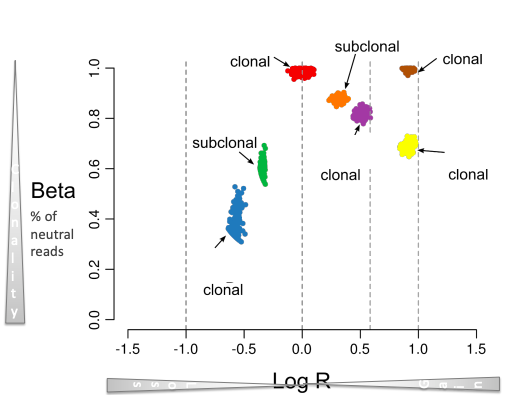
\includegraphics[width=0.5\textwidth]{image2.png} &   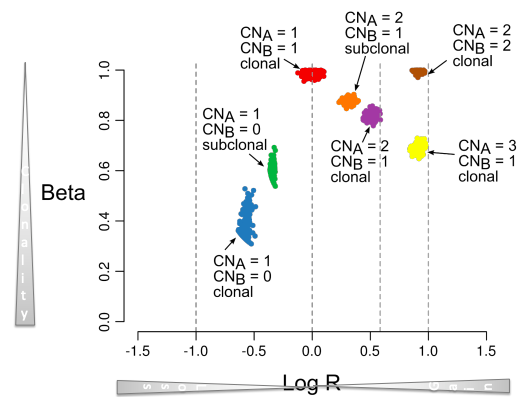
\includegraphics[width=0.5\textwidth]{image3.png} \\
(a) Clonality & (b) CNV \\[6pt]
\end{tabular}
\caption{Lower clusters are more clonal, the more left the deeper they are in terms of loss of DNA.}
\label{fig:cluster}
\end{figure}

Looking at panel A of figure \ref{fig:cluster}
\begin{itemize}
\item The blue cluster with deletions is the most clonal one.
\item Both blue and green clusters have deletions, since they have a negative log2 ratio, but the green one is less clonal than the blue one.
\item In log2 R = 0 and $\beta$ = 1, where there's the red cluster, we have a status of no copy number changes (wild-type status in terms of copy numbers). This basically represents a total number of alleles which is the same in both the tumor and normal sample.
\item All the other clusters with a positive log2 ratio had a gain of DNA.
\end{itemize}

In panel B of figure \ref{fig:cluster} the number of copies that correspond to all the clusters in the space is also reported.

\begin{itemize}
\item Blue: one copy of DNA, so there's a deletion
\item Green one: also one copy of DNA but with subclonality
\end{itemize}

This is how we can map in the space the status of clonality and the number of copies for a specific segment in the genome.


\section{Evolution maps}
We can use the information on clonality to build \textbf{evolution maps}. We wish to track the evolution of tumors over time with specific conditions e.g. treatment.

\subsection{A toy example}
The first thing to do is to look, within each individual, at concomitant deletion where one is subclonal to the other one.

\begin{figure}[H]
\begin{tabular}{cc}
  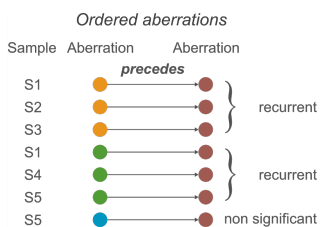
\includegraphics[width=0.5\textwidth]{image4.png} &   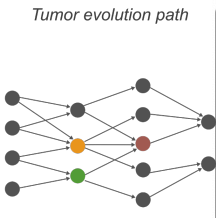
\includegraphics[width=0.5\textwidth]{image5.png} \\
(a) Ordered aberratios & (b) Tumor evolution path \\[6pt]
\end{tabular}
\caption{Lower clusters are more clonal, the more left the deeper they are in terms of loss of DNA.}
\label{fig:evolution}
\end{figure}

In panel A of figure \ref{fig:evolution}:
\begin{itemize}
\item In sample 1 the brown lesion is subclonal to the orange one, and that same lesion is also subclonal to the green one.
\item In sample 2 we have again the support of the relation between the brown and orange lesion with the same level of subclonality (brown subclonal to orange).
\item In sample 3 is the same as in sample 1 and 2.
\item Samples 4 and 5 have the same concomitant green and brown lesions again with the same level of subclonality.
\item In sample 5 only we also have another concomitant lesion (blue subclonal to brown). The blue lesion is not included in the tumor evolution path, as it is not significant - we cannot build an arc.
\end{itemize}

The statistical support of each ‘arrow’ will depend on the number of observations and the total number of co-occurrences.
\\
We then perform this analysis for all the concomitant lesions in our sample and we start drawing edges to keep track of what is subclonal to what. We compile this list across all individuals and look for how many times we see support for the same relationship in the same direction.
\\
In our case we can say that the relationship going from orange to brown is supported by 3 out of 5 individuals; the same can be said for the green going to brown. The blue one is instead not significant since it's supported by only one individual.
\\
So having multiple observation supporting that aberration x precedes aberration y (i.e. aberration y is subclonal to aberration x) we can build an evolution chart.
\\
\\
%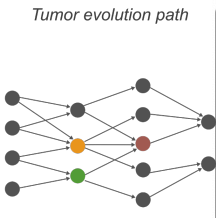
\includegraphics[width=2.38194in,height=2.40417in]{image5.png}\\
In panel B of image \ref{fig:evolution} we have a graph representing the possible tumor evolution path.
The orange and the green which have no relationship between them, are at the same level on the x axis in the path and they both go into brown. So one can assume that the more clonal a lesion is the more likely it is that it occurred earlier during the evolution (time is on the x axis of the path), and we can look for recurrent relationships among lesions.
\\
In principle we can say that the grey ones at the beginning happened at the same time point and then at a second time point, the tumors in our set of samples, underwent loss of orange and green genes and then later they both underwent loss of the brown gene.

\subsection{Working with real data}


\begin{figure}[H]
\centering
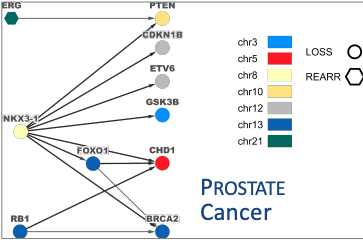
\includegraphics[width=0.5\linewidth]{image6.png}
\caption{}
\label{fig:real}
\end{figure}


If we perform the same analysis in large datasets (lung cancer melanoma, prostate cancer \ldots) we can come up with all the dependencies that were observed and that were supported by more
than one individual (e.g. in prostate cancer we can say that a loss in NKX3-1 precedes the deletion of PTEN).
\\
Even if we have hundreds of BAM files on whole exon sequencing data from large collections all that we can build are evolution maps with at most three layers (pretty disappointing).
\\
One reason for this is that to build a relationship which is statistically significant between two genes we need to have multiple instances of that relationship (in many samples).
Meaning that we need to have co-occurrence of the two lesions and subclonality of the second lesion with respect to the first in a significant number of individuals compared to the total number of individuals that have co-occurrence. 
So if co-occurrence occurs in N individuals and subclonality of the second lesion to the first one occurs in a fraction of those, only if this fraction is significant with a proportion test out of the total number, then we can build the path. We are tremendously limited by co-occurrence of lesions.
\\
\subsection{Pathway based evolution analysis}
To boost the reconstruction of these paths gene families or \textbf{pathways} have been exploited, like for prostate cancer in figure \ref{fig:prostate_path}

\begin{figure}[H]
\centering
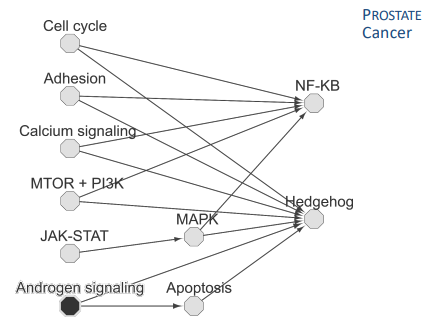
\includegraphics[width=0.4\linewidth]{pathways.png}
\caption{Pathway evolution study example for prostate cancer}
\label{fig:prostate_path}
\end{figure}

E.g. if we are dealing with PTEN, which is a tumor-suppressive gene relevant in a specific pathway (PF3K), then it doesn't matter if we have deletion or inactivation of the same genes in the same pathway, what matters for the tumor evolution is that that specific pathway is altered and so what we can do is start aggregating signals from genes that belong to the same pathway.
\\
So if individual 1 has a relationship between gene A and some gene in a specific pathway (PF3K) and individual 2 has a relationship between gene A and a second gene in that same pathway, then we can assume that maybe they have the same effect and so we can aggregate the information on the landing gene.
\\
Basically, instead of going from gene 1 to gene 2 we go from pathway 1 to pathway 2, and in terms of numbers what we gain is that the co-occurrences are counted including all the gene lesions with the same function in pathway 1 and all the gene lesions with the same function in pathway 2 (if we consider the inactivation of the gene then we have to consider all the lesions that inactivate the gene and not others).
\\
With this method we start having some more data to look for major changes during the evolution of the tumor pathway.

E.g. in prostate cancer we'd identify a set of pathways that are more or less at some level altered in earlier staged disease and that then trigger or are precedent to our pathways. Doing so we can learn more in terms of the biology of the disease evolution.
\\
There are also more complicated ways to make inference of tumor evolution. Some try to avoid the hypothesis that the more clonal a lesion is the more likely it is to happen early, because we know it's not always the case; it might be in untreated samples but not in treated samples. 
In a treatment regiment, because of drug pressure selection, specific resistant clones harboring a specific lesion can take over due to their higher rate of proliferation.
In this case, if we see a lesion that appears to be more clonal, it doesn't really mean that it happened earlier, it may be that it had a higher proliferation and so it's taking over (and we see it as apparently clonal but it's in fact a late event).


\section{Ploidy and purity correction on $\log_2(\frac{T}{N})$ data}
How can we use measure of the tumor purity and the effect of the tumor ploidy? How can we compare two different samples for which we quantify completely different levels of tumor content?
\\
For example, suppose we have a sample a 100\% pure and with 50\% of clonality (a lesion present in 50\% of the cells) and a second sample with a tumor purity of 10\% and a clonality of 100\% (a lesion present in 100\% of the cells). We need to compare numbers without having to convert every time, for every lesion, the depth of the lesion based on the tumor content. 
\\
The accuracy in calls for pure or admixture tissues (with same coverage) is different, we are likely to witness many more FP calls in admixture case. In order to compare, we need to \textbf{adjust the signal} for tumor \textbf{purity} and \textbf{ploidy}. 
\\
The coverage makes data coming from different samples comparable because we normalize everything to the total coverage, but when we deal with diseased cells we can have contamination from the admixture, so we need an extra step. The step, once we know how to assess the tumor purity and ploidy, is quite simple: we need to adjust the data for tumor purity and ploidy. An example is reported in figure \ref{fig:ploidy1}. These corrections are part of standard preprocessing.

\subsection{Melanoma example}

\begin{figure}[H]
\centering
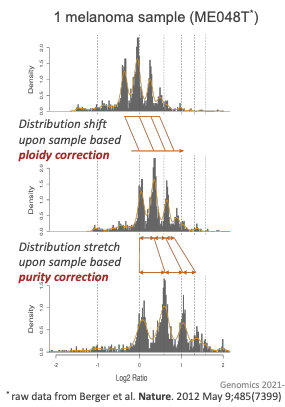
\includegraphics[width=0.4\linewidth]{image7.png}
\caption{Highly aberrant melanoma sample: genome duplication at some point + intervening lesions. The ploidy correction shifts the distribution around zero. For purity correction, the nominal value is around -1→ stretch distribution, set peaks at the right position.
Raw data from Berger et al. Nature. 2012 May 9;485(7399)}
\label{fig:ploidy1}
\end{figure}

In the figure we are looking at one tumor sample: a whole genome sequencing ofone melanoma sample.We see multiple peaks which correspond to different copy number states.
\\
Most of the time, no matter NGS or array data, the best way to detect CNV is to compare tumor signals with normal signals. Image having tumor data with no somatic changes; if we match it to a normal genome, the two samples will be really similar (just some noise). The histogram of the log2ratio will look like a Normal distribution centered around zero.
\\
Instead, when we have a tumor sample with many heterozygous or homozygous deletions; the distribution will still have a bulk around zero, but also two bums towards -1 (first heterozygous, then homozygous deletion). Extra copies would be represented by bums towards +1. In the case of admixture samples, the noise effect will prevent us to clearly identify bums, as they will be closer to the central peak.

Let's suppose we have a genome with a backbone of three copies but we sequence a
bulk and we don't have 100\% purity but 80\% (so 20\% is contamination).

\subsubsection{Ploidy correction}
Computationally we assess the ploidy through the copy number space and then
correct the data.
From the tumor and the match normal we obtain something like the first plot (top-left in picture \ref{fig:ploidy1}, and we could wrongly assume that the main peak is always in 0 (wild-type state of the genome), but it shouldn't.
In fact, if we assess the ploidy and overall we see a backbone state of three copies for our genome, then the main peak should be shifted toward three.
\\
So, the \emph{ploidy correction shifts the distribution} towards the right (second graph, \ref{fig:ploidy1}).

\subsubsection{Purity correction}
We correct our data and the \emph{{purity correction causes a stretch between
the peaks}}, since tumor admixture dilutes the signal. So, the effect of purity
correction is a wider spread between the peaks (third graph, \ref{fig:ploidy1}).

\subsection{Melanoma example with 25 samples}
 If we have one extra copy in our tumor, the log2 ratio will be around 0.58 and so we would expect that the signal will peak around that value; for two extra  copies we'd expect a peak around 1 and so on.
\\
We'll have the peak of the normal state around 0 and then if we have an underrepresented allele in our tumor we'd get another peak around -1 for the hemizygous deletion and then the homozygous deletion.
\\
If our signal is not 100\% pure tumor (so diluted by normal cells), the peak at -1 and 0.5 would be closer to the 0 peak for uncorrected data.


\begin{figure}[H]
\centering
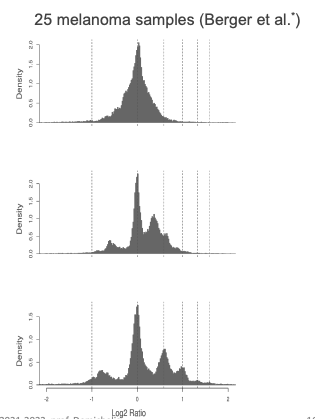
\includegraphics[width=0.4\linewidth]{image8.png}
\caption{25 melanoma samples. Ploidy correction: start seeing interpretable signal. Purity correction: even though it is not perfect (hemizygous is different form -1), it is still quite clear. Raw data from Berger et al. Nature. 2012 May 9;485(7399)}
\label{fig:ploidy2}
\end{figure}

\begin{itemize}
\item
  1\textsuperscript{st} graph (\ref{fig:ploidy2}): the distribution of the log2 data of uncorrected signal, every melanoma sample is highly aberrant with a ploidy that is different between different individuals and a purity that is also different between different individuals. But we do have the tumor ploidy and purity so we can correct the data and get rid of the noise.
\item
  2\textsuperscript{nd} graph (\ref{fig:ploidy2}): we correct for ploidy.
\item
  3\textsuperscript{rd} graph (\ref{fig:ploidy2}): we correct for purity too.
\end{itemize}

From the corrected data we learn that:

\begin{itemize}
\item
  A lot of tumors have a backbone ploidy of two;
\item
  There are some hemyzigous deletion not perfectly centered in one but closer to one in the 3\textsuperscript{rd} graph if compared to the 1\textsuperscript{st};
\item
  Some signal is compatible with homozygous deletion;
\item
  We have a reasonable amount of signal for three copies which could come from a threeploid status of some tumors.
\end{itemize}

\subsection{TCGA example}
%\emph{\textbf{Tumor Ploidy and Purity adjustment, corrected TCGA data}}
How commonly does suboptimal tumor purity affect proper copy number data analysis? How common it is that purity is not equal to 100\% and ploidy is not equal to 2 in any primary disease?

\begin{figure}[H]
\centering
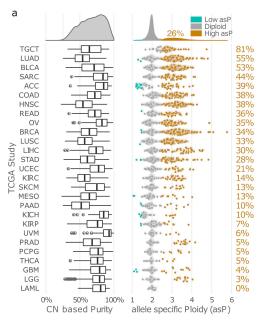
\includegraphics[width=0.5\linewidth]{image9.png}
\caption{}
\label{fig:tcga}
\end{figure}

In figure \ref{fig:tcga} we can see a list of tumor types, where every draw is a tumor type (lung carcinoma, bladder cancer, colon cancer, ovarian ecc.). On the x axis we have tumor purity (1-admixture) going from 0 to 100\% and for each type we can see the distribution of the tumor purity analysis of all the samples from the TCGA dataset. Every tumor type has a different number of sample profile.
\\
Looking at the GBM (glioblastoma multiforme), the middle vertical line is the median signal of the distribution, there are outliers shown and the black horizontal line represents the interquartile range.
\\
Altogether, 8,183 primary cancer samples matched to 27 tumor types profiled with WES from TCGA. 4,950 cases with overall high tumor cellularity were identified. The majority had 69\% tumor purity. There are some outliers e.g. ovarian cancer has high purity.

\subsubsection{Ploidy in TCGA example}
Looking only at ploidy: what is the fraction within each tumor type with a ploidy significantly above two?
\\
In the plot \ref{fig:tcga} they are sorted by decreasing percentage of tumors with a ploidy higher than two; for example, for the first and second tumor type, more than 50
\% of the primary tumors have a ploidy status above two.
Meaning, either they underwent whole genome duplication (4 or more copies) or triplody (3) etc.
\\
Then we have some tumors with very low ploidy (blue dots) where at least one
copy of the entire genome is completely lost - low allele specific
ploidy assessment.
\\
Figure \ref{fig:ploidy_tcga} shows what happens to data when we correct for ploidy and purity.

\begin{figure}[H]
\centering
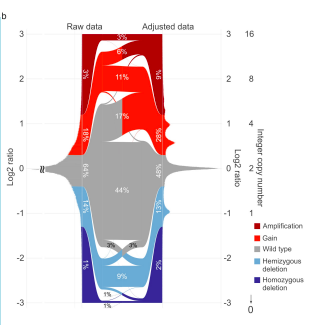
\includegraphics[width=0.5\linewidth]{image10.png}
\caption{Y axis is the log2 ratio. On the left side we have the raw data, On the right side the adjusted data.}
\label{fig:ploidy_tcga}
\end{figure}

We can see where correction for ploidy and purity takes the signal. Focusing just on the first half we can see that we have the same noise we've seen for the melanoma uncorrected data.
\\
The correction of the data results in the reclassification of 30\% of the
totality of the segments (if we don't correct we have a wrong copy number
classification in 30\% of the cases).
\\
What's interesting is that the correction led to the doubling of the homozygous
deletions that we were able to observe (these are very important because it
means that the protein product won't be there at all).

\subsection{Allele-specific analysis}

\begin{figure}[H]
\centering
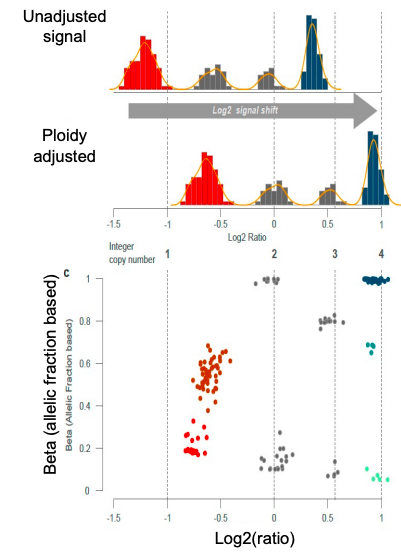
\includegraphics[width=0.5\linewidth]{image11.png}
\caption{Top panel: loss of an allele on A so we'll have 2-1-2 copies. Bottom panel: same situation on allele A but allele B is doubled so we'll have
3-2-3 copies. So, in this situation, the gene x will have two copies but both of them coming
from the same allele (B).
\\
By computing the log2 ratio in this situation we'll have the log2(2/2) which will lead to the collocation on the 0 axis but on the lower part (due to the clonality).}
\label{fig:img11}
\end{figure}

In figure \ref{fig:img11} the data is adjusted. Then samples are represented in the beta-log2 ratio space where we can see that the data underneath the peaks are belonging to specific clusters.
\\
This suggests that by only looking at the log2 ratio we are unable to distinguish the presence of clusters with different clonalities.
\\
The most interesting information is the lower cluster (on the x=0 axis).Even when the T/N = 1 (tumor/normal ratio) there is a status of one copy, and one copy -or something- that equally gives a log2 ratio equal to 0, which still represents copy neutral loss of heterozygosity (CN-LOH), so two copies on one allele and zero copies on the other.
\\
The log2-beta statuses allows us to distinguish the copy-neutral LOH. There are equations that allows us to go from here to a space where our coordinates are the number of copies of allele A and number of copies of allele B, as depicted in figure \ref{fig:img12}.

\begin{figure}[H]
\centering
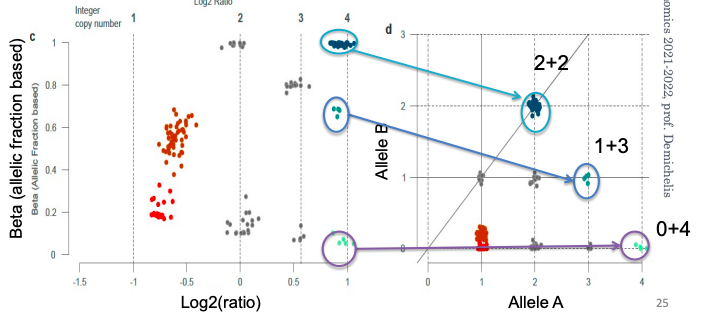
\includegraphics[width=0.5\linewidth]{image12.png}
\caption{}
\label{fig:img12}
\end{figure}

For four copies we can have different combinations:
\begin{itemize}
\item
  2 copies of A + 2 copies of B,
\item
  3 copies of A + 1 copy of B
\item
  4 copies of A + 0 copies of B
\end{itemize}

The equations will not be discussed, what's important is that once we have corrected the data then we can shift our analysis up to the level of number of copies of each allele for each gene.

\emph{Why is this important?}
Let's imagine that for gene X we have one copy lost on allele A and a point mutation on the allele B which leads to unfunctional product so full loss of the protein.
If we instead are in the second case and the point mutation happened after the duplication then we'll still have an allele functioning, whereas if it happened before the duplication, we'd have again full loss of functional protein.
If we are able to distinguish the alleles we are able to also distinguish in which situation we are (which means we can distinguish between what's functional and what's not).

\begin{figure}[H]
\centering
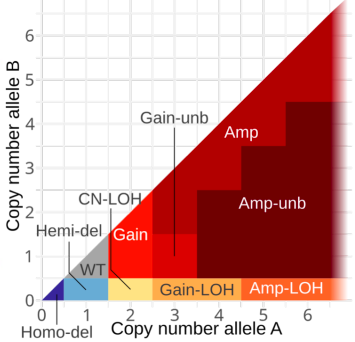
\includegraphics[width=0.3\linewidth]{image13.png}
\caption{Extra graph with the same space allele a/ allele B where we can divide the space in terms of total number of copies and also what happens on both.}
\label{fig:img13}
\end{figure}

So, this whole computation allows us to reclassify copy number status in the space by shifting and stretching and also to assign a copy number A and B to every segment of the genome, which means to every gene.
\\
If we do that we can see that many of the segments that have a total number of copies equal to two are in fact 2+0 and not 1+1. This means that there is a significant fraction of the genome which is apparently wild-type but which actually underwent loss from one an allele and a gain on the other. This event is called copy-neutral loss of heterozygosity (\textbf{CN-LOH}). Copy-neutral because the number of copies doesn't change but there's been loss of heterozygosity.
\\
From the TCGA data, they observed a relevant fraction of high copy number levels
(4-5 copies) which all came from the same allele (one allele was lost and the
other underwent multiple cycles of duplication).

\begin{figure}[H]
\centering
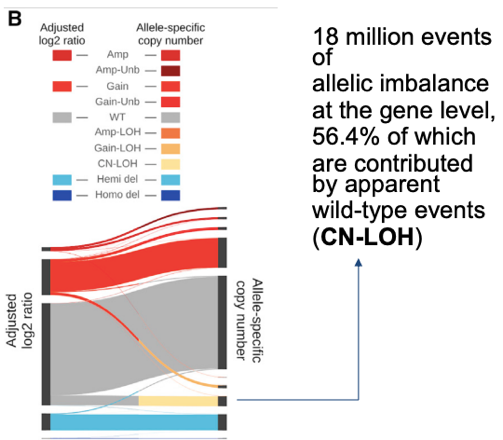
\includegraphics[width=0.5\linewidth]{image14.png}
\caption{Ciani et al, Cell Syst 2022}
\label{fig:img14}
\end{figure}

So, looking at the copy number only we'd say there's a gain (which is true) but we wouldn't have all the complete information (we also have to perform the allele analysis).
\\
This information is relevant in precision medicine because there are ways to target genes exploiting loss of heterozygosity and up until now it was only used for deletions but now that's known, even if we have an apparent CN-LOH or we have a copy number gain LOH we can still consider to use the same approach.

\subsection{A Case study $CN_A$, $CN_B$ real data example}
We have one patient and we're looking at a primary sample, for which we plot the
whole sequencing data in the copy number allele space and what we see (from the
first plot in figure \ref{fig:img15}) is that:

\begin{figure}[H]
\centering
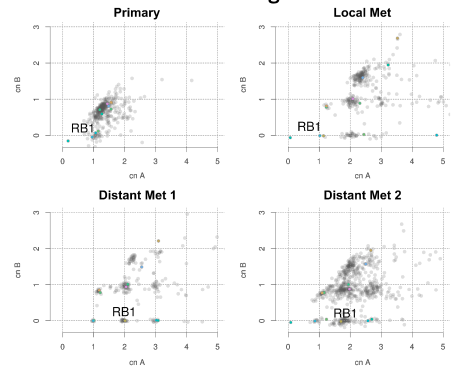
\includegraphics[width=0.7\linewidth]{image15.png}
\caption{Case study - $CN_A$, $CN_B$ real data example with multi-sample data from the same patient. J Clin Invest. 2020 Apr 1;130(4):1653 -1668. doi: 10.1172/JCI131041}
\label{fig:img15}
\end{figure}

\begin{itemize}
\item
  There's a cloud of dots (every dot is a gene) which has a total number of copies around two;
\item
  There's a cluster that underwent hemyzygous deletion so we only have one copy of all the genes in there;
\item
  There's one gene with a homozygous deletion (0,0).
\end{itemize}

Then we have three other metastatic sites for which they had biopsies so that they could run whole genome sequencing and perform the analysis of the data in the same space. We have a local metastasis and two distant mets.

What we see is:
\begin{itemize}
\item
  In distant met 1 there's no homozygous deletion\footnote{How's possible that there's a homozygous deletion in the primary tumor which is then absent in the distant mets?} No DNA can be regained, it's impossible that the gene is reacquired, so probably the seeding of the distant mets happened before the loss of the gene
\item
  In both the distant mets the gene RB1 gained an extra copy on allele A;
\item
  In all the mets there are extra gains of copies of all the genes (maybe there's been a whole genome duplication of some sort);
\item
  In distant met 1 the data are as clean as to allow us to state that the data point in yellow/grey over the 1 is subclonal (if we have genes with 1+1 copy is equivalent to say it's a subclonal hemizygous loss, it means that all the cells have at least one copy and then some cells also have a second copy);
\item
  In terms of evolution, very likely extra copies of the whole genome also in the local met after the loss of the second copy of the gene;
\item
  CN-LOH of many genes, including RB1;
\item
  Level of subclonality overall not high;
\end{itemize}

\subsubsection{Application of longitudinal plasma profiling}
Another way to track evolution is to have \textbf{time points.}
\begin{figure}[H]
\centering
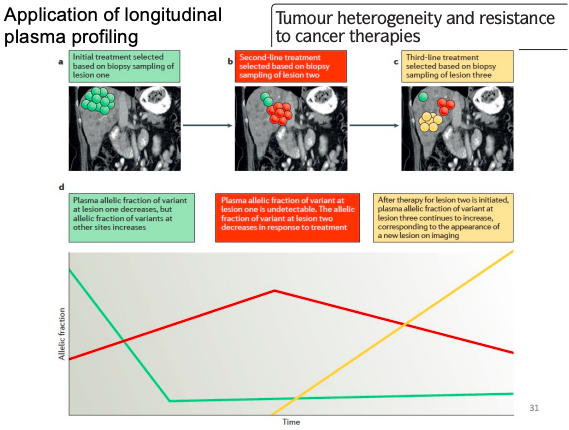
\includegraphics[width=0.8\linewidth]{image16.png}
\caption{\textbf{Application of longitudinal plasma profiling.}Longitudinal monitoring of alterations in circulating tumour DNA has the potential to enable molecular relapses to be detected before the emergence of disease relapse on imaging. In a hypothetical example: \textbf{a)} A biopsy sample from lesion one (green) leads to the use of a targeted agent directed at the alterations in lesion one. \textbf{b)} A failure to also sample lesion two (red) might then lead to outgrowth of clones harbouring alternative molecular alterations, prompting the use of a combination of targeted agents or use of a single targeted therapy capable Of overcoming both molecular alterations. \textbf{c)} The emergence Of lesion three (yellow) might then be
missed by biopsy sampling until this lesion becomes detectable on imaging. \textbf{d)} Longitudinal analysis of liquid biopsy
mples would enable the detection and determination of the allelic fractions of the variants at all three lesions before their detection on imaging. This figure illustrates the ability ofthe molecular analysis of plasma to convey the full spectrum of resistance alterations and shows the dynamic nature of resistance.}
\label{fig:img16}
\end{figure}

If we deal with biopsies over time we can track the evolution using the allelic fraction of a lesion.
Reasoning in terms of point mutations, let's say we have a point mutation at time point 0 in certain allelic fractions, which correspond to different subsets, we track the fractions over time.
\\
Remember: allelic fraction at any time point needs to be corrected for tumor content, otherwise we would not be able to compare multiple time points from the same patient.
